\documentclass[russian,utf8,emptystyle]{eskdtext}

\newcommand{\No}{\textnumero} % костыль для фикса ошибки

\ESKDdepartment{Федеральное государственное бюджетное образовательное учреждение высшего профессионального образования}
\ESKDcompany{Московский государственный технический университет им. Н. Э. Баумана}
\ESKDclassCode{23 0102}
\ESKDtitle{АИС поиска алгоритмов распознавания изоморфизма графов с помощью генетического программирования}
\ESKDdocName{Расчетно-пояснительная записка}
\ESKDauthor{Гуща~А.~В.}
\ESKDtitleApprovedBy{~}{~\underline{\hspace{2.5cm}}}
\ESKDtitleAgreedBy{~}{~\underline{\hspace{2.5cm}}}
\ESKDtitleDesignedBy{Студент группы ИУ5-82}{Гуща~А.~В}

\usepackage{multirow}
\usepackage{tabularx}
\usepackage{tabularx,ragged2e}
\usepackage{pdfpages}
\renewcommand\tabularxcolumn[1]{>{\Centering}p{#1}}
\newcommand\abs[1]{\left|#1\right|}

\usepackage{geometry}
\geometry{footskip = 1cm}

\pagenumbering{arabic}
\pagestyle{plain}

\begin{document}
\includepdf[pages={1}]{title.pdf}

\newpage
\tableofcontents
\newpage

\section{Введение}
Задача проверки изоморфизма графов является актуальной и исключительно привлекательной проблемой в наше время. Нахождение эффективного алгоритма, который за полиномиальное время позволит отвечать на данный вопрос, положительным образом повлияет на такие прикладные задачи как:
\begin{itemize}
\item Поиск химических соединений по базам данных в хемоинформатике и математической химии
\item Верификация различных представлений электронной схемы в автоматизации проектирования электронных схем
\item Выделение общих подвыражений в оптимизации программ
\item Сопоставление графов знаний, содержащихся в семантических сетях
\end{itemize}
Уникальность данной задачи в том, что это одна из двух задач (и одна из 12, перечисленных в \cite{GareyAndJohnson1979}), для которых класс сложности не был определен. Задача проверки изоморфизма графов принадлежит классу NP задач, но не доказано, что она является NP-полной задачей, и не найден алгоритм, решающий ее за полиномиальное время.

В 60-х~--- 80-х годах неоднократно предпринимались попытки решить данную задачу, но они не увенчались успехом. На данный момент лучший алгоритм имеет временную оценку сложности $2^{O(\sqrt{n log(n)})}$ \cite{Johnson2005} \cite{BabaiCodenotti2008}.

В наши дни информационные технологии все больше используются как научные инструменты (яркий пример - решение проблемы четырех красок \cite{FourColourProblem}). С ростом вычислительной мощности растет актуальность использовать автоматические методы поиска решения, например, метод генетического программирования. В данной работе разработан инструмент, спроектированный производить поиск решения задачи проверки отношения изоморфизма для ориентированных графов с выводом преобразованных в графическую форму промежуточных результатов для анализа человеком.

\newpage
\section{Конструкторская часть}
\subsection{Общетехническое обоснование разработки}
\subsubsection{Постановка задачи проектирования}
Задача - разработать автоматизированную информационную систему, реализующую автоматический поиск алгоритмов проверки отношения изоморфизма ориентированных графов и предоставляющую графическую информацию о промежуточных результатах пользователю для анализа.

Задачи проектирования могут быть сформулированы следующим образом:
\begin{enumerate}
\item Исследование предметной области проектирования
\item Определение функциональных задач
\item Изучение метода <<Генетическое программирование>>
\item Разработка проблемно-ориентированного языка для внутреннего представления программ
\item Выбор и обоснование критериев качества программы и оценки работы найденных алгоритмов
\item Разработка схемы данных
\item Разработка алгоритмов программы
\item Разработка программы
\item Отладка программы
\item Разработка графического интерфейса пользователя
\item Тестирование программы
\item Разработка конструкторской и эксплуатационной документации
\end{enumerate}

\subsubsection{Описание предметной области}
\textbf{Ориентированный граф} - совокупность непустого множества вершин и множества связей между вершинами, называемыми ребрами. Ребра являются упорядоченными парами вершин.

\begin{align*}
G &\equiv ( E, V ) \\ 
V &\equiv \{ (e_1, e_2) | e_1 \in E \wedge e_2 \in E \}
\end{align*}

$e_1$ - \textbf{начало} ребра, $e_2$ - \textbf{конец} ребра. Далее ребро будет обозначаться следующем образом:
$$
v = e_1 \rightarrow e_2
$$
Далее рассматриваются только графы с конечным множеством вершин и ребер.

Граф $G$ называется \textbf{изоморфным} графу $H$, если существует биекция $f$ из множества вершин графа $G$ в множество вершин графа $H$, обладающая следующим свойством: если в графе $G$ есть ребро из вершины $A$ в вершину $B$, то в графе должно быть ребро из вершины $f(A)$ в вершину $f(B)$ и наоборот --- если в графе $H$ есть ребро из вершины $A$ в вершину $B$, то и в графе $G$ должно быть ребро из вершины $f^{-1}(A)$ в вершину $f^{-1}(B)$. Биекция также должна сохранять ориентацию ориентированного графа.

\begin{figure}[h!]
\centering
\includegraphics[scale=0.6]{graphs_isomorph_example_1}
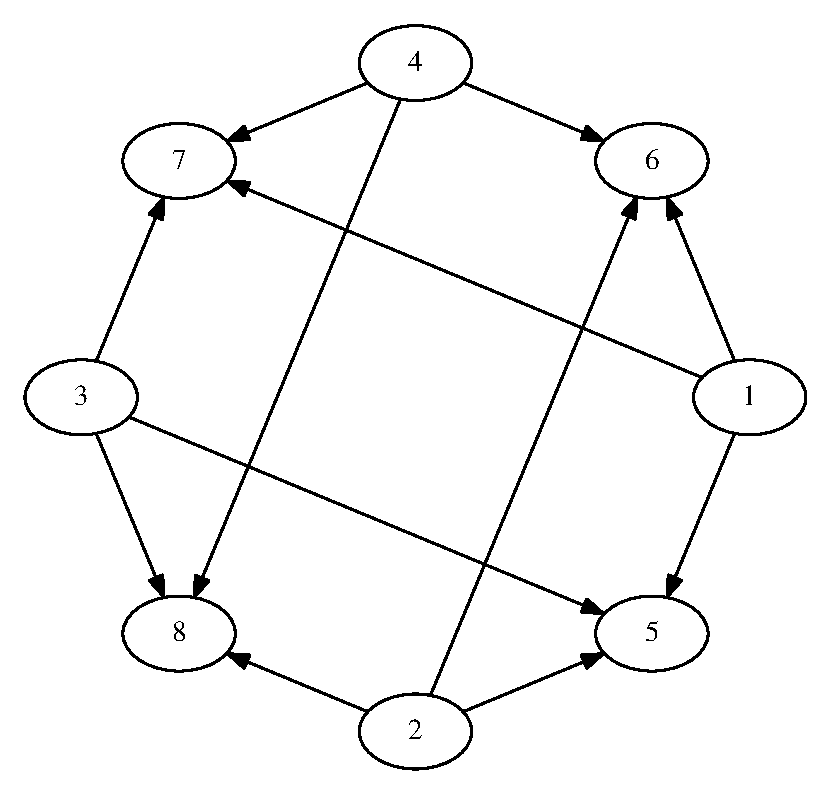
\includegraphics[scale=0.6]{graphs_isomorph_example_2}
\caption{Пример изоморфных графов}
\end{figure}

\textbf{Матрица смежности графа $G$ с конечным числом вершин $n$} - это квадратная матрица $A$ размера $n$, в которой значение элемента $a_{ij}$ равно числу ребер из $i$-й вершины графа в $j$-ю вершину. 

Самый прямолинейный способ установить отношение изоморфности между графами $G$ и $H$ - перестановками строк и столбцов матрицы смежности графа $G$ получить матрицу смежности графа $H$. Однако перебор всех возможных перестановок характеризуется вычислительной сложностью $O(N!)$, что практически исключает применение подобного подхода на практике.

Существует набор числовых характеристик графов, называемыми полными инвариантами, совпадение которых у различных графов является необходимым и достаточным условием изоморфизма. Примерами таких инвариантов являются:
\begin{itemize}
\item Мини-код $\mu_{min}(G)$ матрицы смежности, получаемый путем выписывания двоичных значений матрицы смежности в строчку с последующим переводом полученного двоичного числа в десятичную форму. Мини-коду соответствует такой порядок следования строк и стобцов, при котором полученное значение является минимально возможным.
\item Макси-код $\mu_{max}(G)$ матрицы смежности, получаемый путем выписывания двоичных значений матрицы смежности в строчку с последующим переводом полученного двоичного числа в десятичную форму. Макси-коду соответствует такой порядок следования строк и стобцов, при котором полученное значение является максимально возможным.
\end{itemize}

В настоящее время полный инвариант графа, вычислимый за полиномиальное время, неизвестен, однако не доказано, что он не существует. Попытки его отыскания неоднократно предпринимались в 60-х~--- 80-х годах XX века, однако не увенчались успехом. На данный момент лучший алгоритм определения изоморфизма графов имеет временную оценку сложности $2^{O(\sqrt{n log(n)})}$ \cite{Johnson2005} \cite{BabaiCodenotti2008}.

\subsubsection{Перечень процессов, подлежащих автоматизации}
Процессы, которые подлежат автоматизации:
\begin{enumerate}
\item Генерация первичных алгоритмов проверки изоморфизма графов
\item Эволюционный поиск и отбор наилучших алгоритм проверки изоморфизма графов
\item Качественная оценка полученных алгоритмов проверки изоморфизма графов
\item Визуализация полученных алгоритмов проверки изоморфизма графов
\end{enumerate}

\subsubsection{Выбор и обоснование критериев качества}

\subsubsection{Анализ аналогов и прототипов}

\newpage
\subsection{Разработка программного изделия}
\subsubsection{Разработка структуры программного изделия}

\subsubsection{Особенности выбранных технологий}

\subsubsection{Архитектруа программы. UML-диаграмма классов}

\subsubsection{Выбор программных средств}

\subsubsection{Выбор аппаратных средств}

\subsubsection{Разработка основных алгоритмов обработки информации}

\newpage
\subsection{Технологическая часть}
\subsection{Разработка интерфейса взаимодействия с пользователем}

\subsection{Разработка форматов входных и выходных данных программы}
\subsubsection{Разработка форм входных данных}

\subsubsection{Разработка форм выходных данных}

\newpage
\section{Исследовательская часть}

\newpage
\section{Заключение}

\newpage
%\addcontentsline{toc}{chapter}{\bibname}
\bibliographystyle{utf8gost705u}  %% стилевой файл для оформления по ГОСТу
\bibliography{biblio}     %% имя библиографической базы (bib-файла) 

\end{document}